\documentclass{beamer}
\beamertemplatenavigationsymbolsempty
\usecolortheme{beaver}
\setbeamertemplate{blocks}[rounded=true, shadow=true]
\setbeamertemplate{footline}[page number]

\usepackage{amsmath,amssymb,amsfonts}
\usepackage{graphicx}
\usepackage{tikz}

\title{Understanding Invariance via Feedforward Inversion of Discriminatively Trained Classifiers}
\author{Piotr Teterwak, Chiyuan Zhang, Dilip Krishnan, Michael C. Mozer}
\institute{Talk by Dmitry Vasilenko}
\date{}

\begin{document}

\begin{frame}
\titlepage
\end{frame}

\begin{frame}{Problem Statement and Motivation}

Discriminative models should be invariant to irrelevant features, yet...


\begin{itemize}
    \item Classifier: $\Phi: \mathcal{X} \rightarrow \mathbb{R}^{C}$
    \item Logits: $z = \Phi(x)$
    \item Invariance: $\Phi(T(x)) \approx \Phi(x)$ for class-preserving transformations $T$
\end{itemize}

\begin{alertblock}{Key Research Question}
How much information about $x$ is preserved in $z$?
\end{alertblock}
\end{frame}

\begin{frame}{Related Research: Feature Inversion Methods}
\begin{block}{Two Main Approaches for Representation Inversion}

\begin{columns}[T]
\begin{column}{0.48\textwidth}
\centering
\textbf{Optimization-Based Methods}
\begin{itemize}
\item Gradient descent in image space
\item Minimize: 
\small
$L(x, x_0) = ||\Phi(x) - \Phi(x_0)||^2 + \lambda R(x)$
\normalsize

\end{itemize}

\begin{alertblock}{Drawbacks}
\begin{itemize}
\item Sensitive to initialization
\item Requires careful tuning of $\lambda$
\item Slow iterative process
\end{itemize}
\end{alertblock}
\end{column}

\begin{column}{0.48\textwidth}
\centering
\textbf{Learning-Based Methods}
\begin{itemize}
\item Train decoder network on $\{$logits, pixels$\}$ pairs
\item Feedforward inference after training

\end{itemize}

\begin{exampleblock}{Evolution}
\begin{itemize}
\item Initial: Pixel loss + image prior → blurry
\item Improved: + Adversarial loss → better quality
\item \textbf{Our work:} + Conditional projection + Conditional BN
\end{itemize}
\end{exampleblock}
\end{column}
\end{columns}

\end{block}

\end{frame}

\begin{frame}{Method: Architecture Overview}

\begin{figure}
    \centering
    
\includegraphics[width=0.8\linewidth]{1.png}
    \caption{Architecture}
    \label{fig:placeholder}
\end{figure}

\begin{block}{GAN with Logit Conditioning}
\begin{itemize}
    \item Generator: $\hat{x} = G(z, \epsilon)$, $\epsilon \sim \mathcal{N}(0,I)$
    \item Discriminator: $D(\bar{x}, z)$
\end{itemize}
\end{block}
\end{frame}

\begin{frame}{Mathematical Framework: Generator}
\begin{block}{Conditional Batch Normalization}
\begin{equation*}
y'_{l,k} = \gamma_{l,k}(z) \cdot \frac{y_{l,k} - \mathbb{E}[y_{l,k}]}{\sqrt{\mathbb{V}[y_{l,k}]}} + \beta_{l,k}(z)
\end{equation*}
\end{block}

\begin{block}{Parameterization}
\begin{itemize}
    \item $\gamma_{l,k}(\cdot), \beta_{l,k}(\cdot)$ — MLPs mapping from $z$
    \item Logits control "style" at all abstraction levels
\end{itemize}
\end{block}
\end{frame}

\begin{frame}{Mathematical Framework: Discriminator}
\begin{block}{Projection Discriminator}
\begin{equation*}
D(\bar{x}, z) = (w_1 + W_2 z)^\top \Psi(\bar{x})
\end{equation*}
\end{block}

\begin{block}{Components}
\begin{itemize}
    \item $\Psi(\bar{x})$ — image feature vector
    \item $w_1^\top \Psi(\bar{x})$ — "realism" assessment
    \item $(W_2 z)^\top \Psi(\bar{x})$ — "consistency" assessment
\end{itemize}
\end{block}
\end{frame}

\begin{frame}{Loss Function}
\begin{block}{Minimax Objective}
\begin{align*}
\mathcal{L}_D &= \mathbb{E}_{x,\epsilon}[\max(-1, D(G(z,\epsilon), z)) - \min(1, D(x,z))] \\
\mathcal{L}_G &= -\mathbb{E}_{x,\epsilon}[D(G(z,\epsilon), z)]
\end{align*}
\end{block}

\begin{block}{Key Advantages}
\begin{itemize}
    \item Single loss term — no hyperparameter balancing
    \item Feedforward inference — fast reconstruction
\end{itemize}
\end{block}
\end{frame}

\begin{frame}{Method Comparison}

\begin{figure}
    \centering
    
\includegraphics[width=0.5\linewidth]{3.png}
    \caption{Caption}
    \label{fig:placeholder}
\end{figure}

\end{frame}

\begin{frame}{Human Evaluation Results}

\begin{table}[h!]
\centering
\begin{tabular}{lcc}
\hline
\textbf{Comparison} &  & \\
\hline
Ours (Robust ResNet) vs D\&B Robust & 87.5\% & 12.5\% \\
Ours (Robust) vs Ours (Non-Robust) & 76.5\% & 23.5\% \\
Ours (ResNet) vs Ours (Inception) & 52.7\% & 47.3\% \\
\hline
\end{tabular}
\end{table}

\end{frame}


\begin{frame}{Visualizing Model Invariances}

\begin{figure}
    \centering
    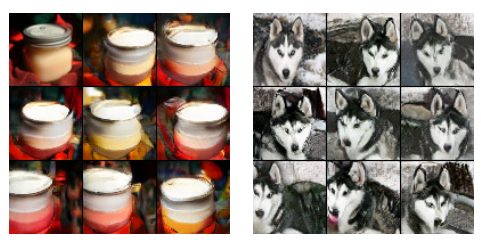
\includegraphics[width=0.55\linewidth]{5.png}
    \caption{Robust ResNet-152}
    \label{fig:placeholder}
\end{figure}

\begin{figure}
    \centering
    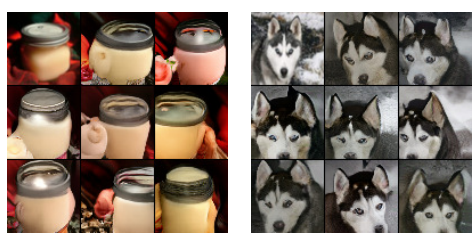
\includegraphics[width=0.55\linewidth]{6.png}
    \caption{non-robust ResNet-152}
    \label{fig:placeholder}
\end{figure}

\end{frame}


\begin{frame}{Reconstructing incorrectly classified images}
\begin{figure}
    \centering
    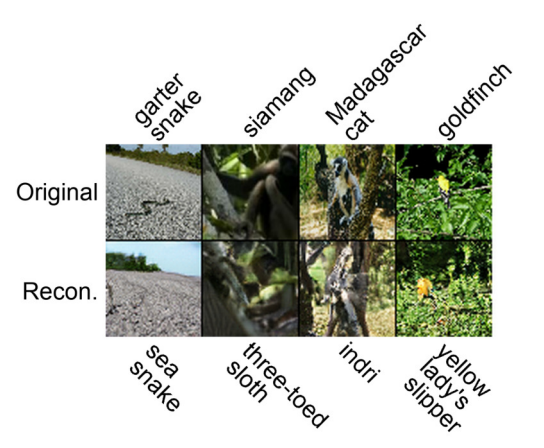
\includegraphics[width=0.9\linewidth]{4.png}

    \label{fig:placeholder}
\end{figure}
\end{frame}

\begin{frame}{Logit manipulations}
\begin{figure}
    \centering
    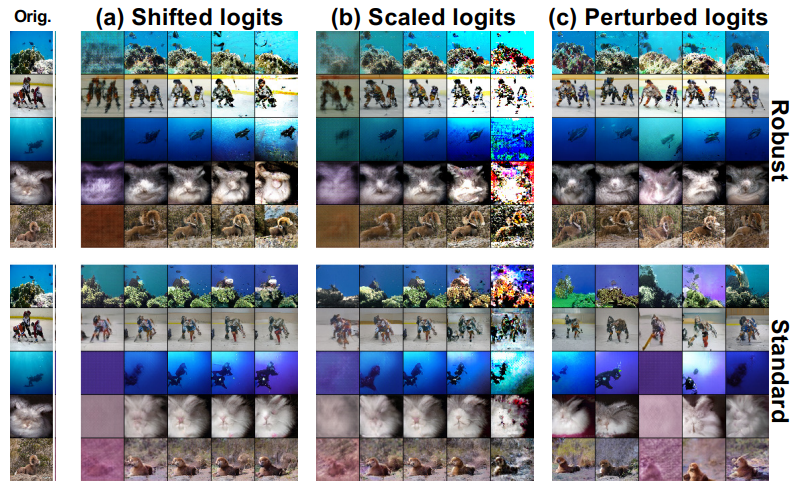
\includegraphics[width=1.1\linewidth]{7.png}
    \label{fig:placeholder}
\end{figure}
\end{frame}


\begin{frame}{Conclusion}

\begin{itemize}
    \item We obtain remarkably high fidelity reconstructions,
which allow the object class to be determined as well
as visual detail orthogonal to the class label.
    \item Robust ResNet produces better reconstructions than non-robust ResNet
    \item Architecture matters. ResNet seems to better preserve
visual information than Inception
    \item We do not see a qualitative difference in reconstruction
fidelity for incorrectly classified images.
    \item For a robust ResNet-152, both logit shifts and rescaling
have have a similar effect—they influence the contrast,
sharpness, and brighness of reconstructions. The relationship for non-robust ResNet is similar but weaker
\end{itemize}



\end{frame}



\end{document}